\documentclass[french]{beamer}
\usepackage[utf8]{inputenc}
\usepackage[T1]{fontenc}

\usepackage{amsmath}
\usepackage{amsfonts}
\usepackage{amssymb}
\usepackage{xcolor}
\usepackage{alltt}
\usepackage{textcomp}
\usepackage{mathrsfs}
\usepackage{stmaryrd}
%\usepackage{subfig}
\usepackage{subfigure}
\usepackage{listings}
\usepackage{pgf}
\usepackage{graphicx}
\usepackage{enumitem}

%\usepackage{fourier}

\usepackage{tikz}
\usetikzlibrary{calc,arrows,patterns,plotmarks,shapes,snakes,er,3d,automata,backgrounds,topaths,trees,petri,mindmap}
\usepackage{pgfplots}
\usepackage{pgfplotstable}

%%% For code c++ environment
\definecolor{blue_code}{RGB}{106, 90, 205}
\definecolor{grey_comment}{RGB}{105, 105, 105}

\usepackage{filecontents,listings}
\lstset{language=c++,showspaces=false,showstringspaces=false,captionpos=t,literate={>>}{\ensuremath{>>}}1,mathescape}
\lstset{basicstyle=\small\bf\ttfamily}
\lstset{lineskip=-2pt}

%\lstset{emph={inline},emphstyle=\color{red}\bfseries}

\definecolor{cgreen}{rgb}{0.,0.6,0.0}

\definecolor{violet}{rgb}{0.5,0,0.5}
\definecolor{vertfonce}{rgb}{0.,0.5,0.}
\definecolor{rouge}{rgb}{0.5,0.,0.}
\definecolor{bleu}{rgb}{0.,0.,1}
\definecolor{orange}{rgb}{1,0.5,0}
\lstset{keywordstyle=\color{red}\bfseries}
\lstset{
emph={form,form1,form2,integrate,on,grad,gradt,dot,id,dx,dy,dz,idt,dxt,dyt,dzt,idv,dxv,dy,dzv,gradv,div,divt,divv,dn,jump,trans,vec,cst,
  project,P,Px,Py,Pz,one,oneX,oneY,oneZ,hFace,N,Nx,Ny,Nz,sin,cos,min,max,abs,pow,chi,exp,LinearForm,BilinearForm,MixedLinearForm,MixedBilinearForm,
  FESpace,MixedFESpace,integrate,project,addCL},emphstyle=\color{bleu},
emph={[2]\_space,\_range,\_expr,\_quad,\_quad1,\_test,\_trial,\_matrix,\_vector,\_solution,\_element,\_rhs,\_rowstart,\_colstart,\_block,
  \_pattern,\_pattern\_block,\_domainSpace,\_imageSpace,\_mesh,\_name,\_partitions,\_worldcomm,\_worldscomm,
  \_type,\_marker1,\_marker2,\_marker3,\_marker4,\_marker5,\_marker6,\_marker7,\_marker8,\_markerAll,\_argc,\_argv,\_desc},emphstyle={[2]\color{violet}\bfseries},
emph={[3]elements,markerName,boundaryfaces,markedfaces,\_Q,solve, newMatrix,newVector,newZeroMatrix,newZeroVector,
  newBlockMatrix,newBlockVector,localize,element,apply,createMesh,localSize,subWorldComm,transpose,setMarker,add,save,
  dirichlet\_vec,neumann\_scal,updateTime,exportResults,updateBdf,init,FluidMechanics}, emphstyle={[3]\color{rouge}\bfseries},
emph={[4]Backend,BlocksVector,BlocksSparseMatrix,BlocksStencilPattern,Blocks,opInterpolation,FunctionSpace,Lagrange,bases,Pch,unitSquare,WorldComm,
  Mesh,Simplex,Node,Rectangle,Quadrangle,Circle,AppliManagement,Environment,feel\_options,exporter},emphstyle={[4]\color{orange}\bfseries},
emph={[5]size\_type,uint16\_type},emphstyle={[5]\color{red}\bfseries},
emph={[6]GeoTool,vf,cl},emphstyle={[6]\color{cyan}\bfseries}
}


\lstset{commentstyle=\ttfamily\color{cgreen}}
\lstset{numberstyle=\tiny}
%\lstset{backgroundcolor=\color{lbcolor},rulecolor=}

\lstset{frame=single,framerule=0.5pt}
\lstset{belowskip=\smallskipamount}
\lstset{aboveskip=\smallskipamount}
\lstset{includerangemarker=false,rangeprefix=\/\/\#\ ,% curly left brace plus space
  rangesuffix=\ \#}
%%%%
\usetheme{CambridgeUS}

\title[SEME 2014 - cerema 2]{Utilisation de l'équation de transport pour la prévision du bruit}
\subtitle{Vers un nouveau modèle d'acoustique du batiment}

\author[shortname]{author1 \inst{1} \and author2 \inst{2}}
\institute[shortinst]{\inst{1} affiliation for author1 \and %
                      \inst{2} affiliation for author2}

\titlegraphic{
\includegraphics[width=4cm]{Figures/logo-cerema.jpg} }

\AtBeginSubsection[]{
   \begin{frame}
   \tableofcontents[currentsection,currentsubsection]
   \end{frame} 
}

\begin{document}

\begin{frame}
\titlepage
\end{frame}

\section{Approche numérique}

\subsection{Transport avec une direction fixée pour $\vec{v}$}
\begin{frame}{Equation de transport - Discrétisation}

  \begin{block}{Equation de transport}
    \begin{equation*}
      \frac{\partial w(\vec{r}, \theta, \phi, t)}{\partial t} = -\vec{v} \cdot \nabla w(\vec{r}, \theta, \phi, t) - M v w(\vec{r}, \theta, \phi, t) + 
      w_{sce}(\vec{r}, \theta, \phi, t)
    \end{equation*}
    
    \begin{columns}[c]
      \begin{column}{5cm}
        \begin{itemize}
        \item $\vec{r} : (x_1,...,x_{dim})$ \\
          1D,2D, ou 3D en espace
        \end{itemize}
      \end{column}
      \begin{column}{5cm}
        \begin{itemize}
        \item $\vec{v} : (\theta, \phi)$ \\
          2D pour les directions
        \end{itemize}
      \end{column}
    \end{columns}

    \begin{center}
      \textcolor{red}{Modèle 5D instationnaire}
    \end{center}
  \end{block}

  \begin{alertblock}{Discrétisation : Schéma différence finies implicite centré}
    \begin{columns}[c]
      \begin{column}{6cm}
        \begin{equation*}
          \frac{\partial w}{\partial t} = \frac{w^{t+1}_{\vec{r}} - w^t_{\vec{r}}}{\Delta t}
        \end{equation*}
      \end{column}
      \begin{column}{6cm}
        \begin{equation*}
          \frac{\partial w}{\partial x_i} = \frac{w^{t+1}_{r_i + 1} - w^{t+1}_{r_i - 1}}{2\Delta x_i}
        \end{equation*}
      \end{column}
    \end{columns} 

  \end{alertblock}

\end{frame}

\begin{frame}{Schéma aux différences finies}
  \begin{equation*}
    \frac{w_{\vec{r}}^{t+1} - w_{\vec{r}}^{t}}{\Delta t} + 
    \sum \limits_{i=1}^{Dim} v_i \left( \frac{w_{r_i+1}^{t+1} - w_{r_i-1}^{t+1}}{2 \Delta x_i} \right)
    + Mvw_{\vec{r}}^{t+1} = w_{sce}
  \end{equation*}

  %forme matricielle
  \begin{columns}[c]
    \begin{column}{5cm}
      \centering
      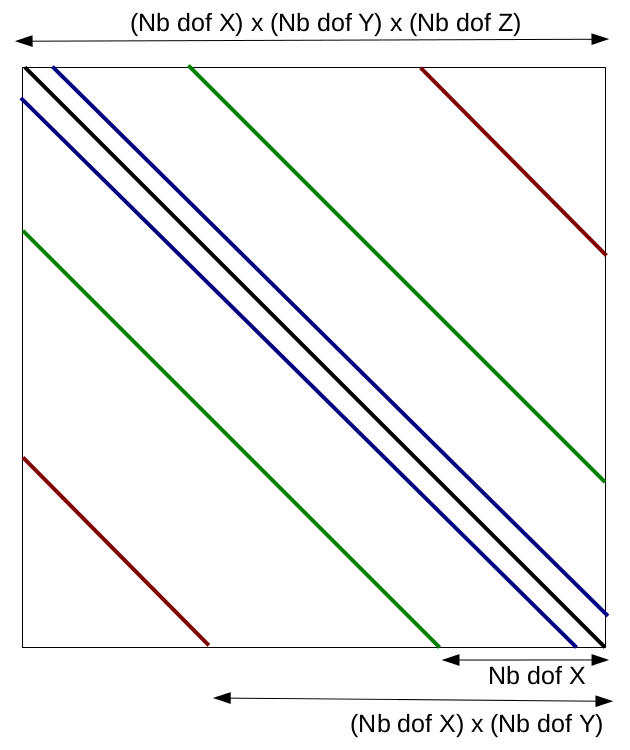
\includegraphics[scale=0.3]{Figures/FD_matrix.png}
    \end{column}
    \begin{column}{6.5cm}
      \begin{itemize}[label=$\rightarrow$]
      \item \textcolor{black}{$\bullet$} terme diagonal : $\frac{1}{\Delta t} + Mv$
      \item \textcolor{blue}{$\bullet$} schéma centré en $x$ : $\pm \frac{v_x}{2\Delta x}$
      \item \textcolor{green}{$\bullet$} schéma centré en $y$ : $\pm \frac{v_y}{2\Delta y}$
      \item \textcolor{red}{$\bullet$} schéma centré en $z$ : $\pm \frac{v_z}{2\Delta z}$
      \end{itemize}
    \end{column}
  \end{columns} 

\end{frame}

\begin{frame}
  Video 1D Dirichlet homogene sans stabilisation
\end{frame}

\begin{frame}{Stabilisation : ajout d'un terme de diffusion artificiel}
  %Stabilisation : ajout d'un terme de diffusion artificiel
  \vspace*{-0.6cm}
  \begin{eqnarray*}
    \frac{\partial w(\vec{r}, \theta, \phi, t)}{\partial t} &=& -\vec{v} \cdot \nabla w(\vec{r}, \theta, \phi, t) - M v w(\vec{r}, \theta, \phi, t) + 
    w_{sce}(\vec{r}, \theta, \phi, t) \\
    &+& \text{ \textcolor{red}{$\nabla (\tau_{art} \nabla w(\vec{r}, \theta, \phi, t))$} } 
    \qquad \tau_{art} = \frac{\rho h \prod \limits_{i=1}^{Dim} v_i }{\parallel \vec{v} \parallel}
  \end{eqnarray*}

  %avec $\tau_{art} = \frac{\rho h \prod \limits_{i=1}^{Dim} v_i }{\parallel \vec{v} \parallel}$

  \vspace*{-0.3cm}
  %forme matricielle
  \begin{columns}[c]
    \begin{column}{4.5cm}
      \centering
      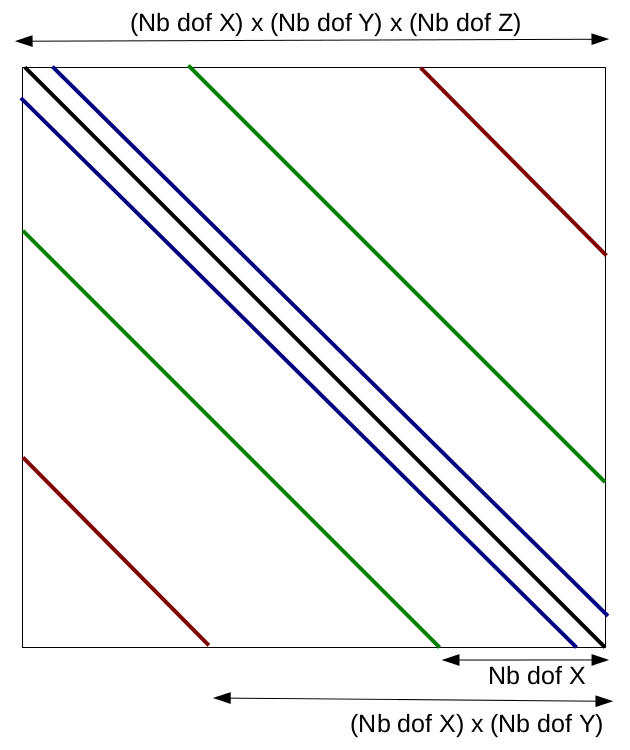
\includegraphics[scale=0.26]{Figures/FD_matrix.png}
    \end{column}
    \begin{column}{7.5cm}
      \begin{itemize}[label=$\rightarrow$]
      \item \textcolor{black}{$\bullet$} terme diagonal : $\frac{1}{\Delta t} + Mv$ 
        + \textcolor{red}{$\frac{2\tau_{art}}{\Delta x^2} + \frac{2\tau_{art}}{\Delta y^2} + \frac{2\tau_{art}}{\Delta z^2}$}
      \item \textcolor{blue}{$\bullet$} schéma centré en $x$ : $\pm \frac{v_x}{2\Delta x}$
        - \textcolor{red}{$\frac{\tau_{art}}{\Delta x^2}$}
      \item \textcolor{green}{$\bullet$} schéma centré en $y$ : $\pm \frac{v_y}{2\Delta y}$
        - \textcolor{red}{$\frac{\tau_{art}}{\Delta y^2}$}
      \item \textcolor{red}{$\bullet$} schéma centré en $z$ : $\pm \frac{v_z}{2\Delta z}$
        - \textcolor{red}{$\frac{\tau_{art}}{\Delta y^2}$}
      \end{itemize}
    \end{column}
  \end{columns} 

\end{frame}

\begin{frame}
  Video 1D Dirichlet homogene avec stabilisation
\end{frame}

\subsection{Prise en compte de la condition limite}
\begin{frame}{Condition aux limites}

  Sur les bords du domaine (= murs de la salle) :
  \begin{itemize}[label=$\bullet$]
  \item une partie de l'énergie est réfléchie de façon spéculaire %(probabilité $1-d$)
  \item l'autre partie est réfléchie de façon diffuse %(probabilité $d$) \\
    \vspace*{0.2cm}
  \item $R$ (coefficient de réflexion) et $d$ (coefficient de diffusivité) dépendent de la paroi considérée
  \end{itemize}

  \vspace*{-0.4cm}
  \begin{small}
    \begin{equation*}
      w(\vec{r},\theta,\phi,t) = \underbrace{R(1-d)w(\vec{r},\hat{\theta},\hat{\phi},t)}_{\text{reflexion spéculaire}}
      + \underbrace{ \int_{0}^{2\pi} \int_{0}^{\frac{\pi}{2}} Rd\frac{1}{\pi v} \vec{v}'w(\vec{r},\theta',\phi',t) sin \theta' d\theta' d\phi'}_{\text{reflexion diffuse}}
    \end{equation*}
    si $\vec{v} \cdot \vec{n} < 0$ ( $w(\vec{r},\theta,\phi,t)$ = 0 sinon) \\
  \end{small}

  où $\vec{v} \cdot \vec{n} = -\hat{\vec{v}} \cdot \vec{n}$, avec
  \begin{equation*}
    v=
    \left(
    \begin{array}{lll}
      cos(\theta)\\
      sin(\theta)cos(\phi)\\
      sin(\theta)sin(\phi)
    \end{array}
    \right)
    \Rightarrow
    \left \{
    \begin{array}{ll}
      \hat{\theta} = \pi - \theta \\
      \hat{\phi} = \pi - \phi \\
    \end{array}
    \right.
  \end{equation*}
  et $\vec{v} \cdot \vec{n} \neq -\vec{v}' \cdot \vec{n}$
\end{frame}

\subsection{Transport prenant en compte plusieurs directions pour $\vec{v}$}
\begin{frame}{Stratégie}

  \begin{columns}[c]
    \begin{column}{6cm}
      \begin{itemize}[label=$\bullet$]
      \item Directions $(\theta,\phi)$ organisées selon une grille 2D
      \item Resolution 3D pour chaque direction $(\theta,\phi)$
      \item \textbf{Résultat} : somme des densités dans toutes les directions :\\
        $w(\vec{r},t) = \sum \limits_{(\theta,\phi)} w(\vec{r},\theta,\phi,t)$
      \end{itemize}

      \begin{alltt}
        for[ pas de temps $t$ ] \\        
        \hspace*{0.2cm} for[ direction $(\theta,\phi)$ ] \\
        \hspace*{0.4cm} assemblage matrice
        \hspace*{0.4cm} assemblage second membre
        \hspace*{0.4cm} Resolution $\Rightarrow w(\vec{r},\theta,\phi,t)$
        \hspace*{0.4cm} $w(\vec{r},t)$ += $w(\vec{r},\theta,\phi,t)$
      \end{alltt}
    \end{column}
    \begin{column}{6.5cm}
      \begin{figure}[H]
        \centering
        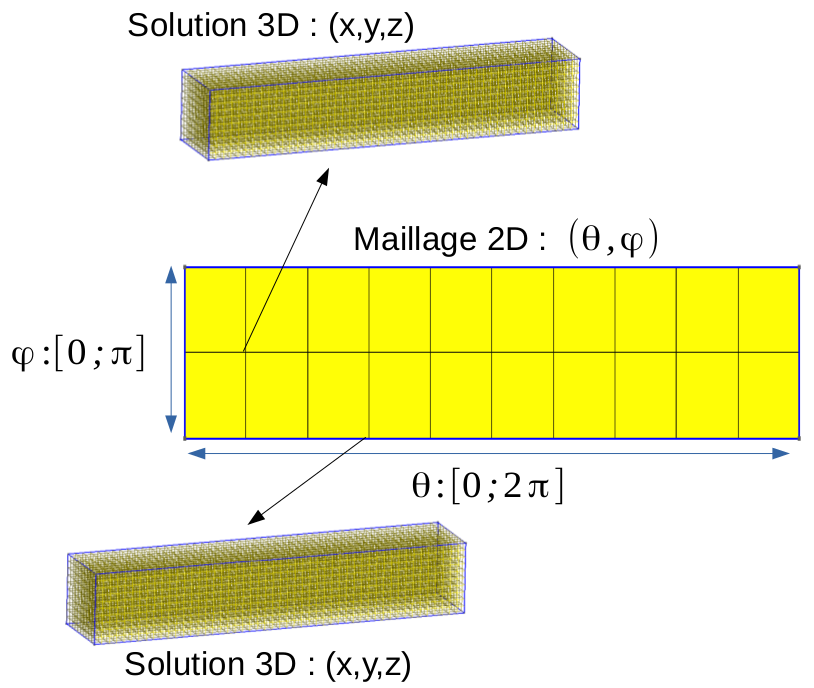
\includegraphics[scale=0.32]{Figures/Schema_mesh.png}
      \end{figure}
    \end{column}
  \end{columns}
\end{frame}





\subsection{Implémentation}
\begin{frame}{Outils numériques : Feel++ }

  \begin{itemize}
  \item Méthode de Galerkin d'ordre arbitraire (cG, dG) en 1D, 2D et 3D% Supports generalized arbitrary order Galerkin methods (cG, dG) in 1D, 2D and 3D
    %\item Supporte les maillages d'ordre élevé (simplex, hypercube)
    %\item Supports generalized arbitrary order Galerkin methods (cG, dG) in 1D, 2D and 3D
    %\item Supports simplex, hypercube, high order meshes and geometries
  \item Langage très proche des mathématiques (DSEL in C++)
    %$\Longrightarrow$ DSEL  (FreeFem++)
    \begin{itemize}
    \item Expressivité : { \scriptsize modèles physiques et méthodes numériques (\alert{haut niveau})} \\
    \item Efficacité : { \scriptsize assemblages et résolutions algébriques (\alert{bas niveau})}
    \end{itemize}
  \end{itemize}


      \begin{columns}
        \column[c]{.4\textwidth}
        \scriptsize
        \vspace*{-0.07\textwidth}

        \begin{eqnarray*}
          \left\{
          \begin{aligned}
            \text{Trouver } &u \text{ qui vérifie :} \quad\quad \\
            -\Delta u &= 1 \ \ \text{dans} \ \Omega \\
            u &= 0 \ \ \text{sur} \ \partial\Omega
          \end{aligned}
          \right. \\
          \fbox{$\underset{\text{variationnelle}}{\overset{\text{Formulation}}{\Longrightarrow}}$} \quad\quad\quad\quad \\
          \left\{
          \begin{aligned}
            \text{Trouver } &u\in V_h \text{ tel que } \\
            \int_\Omega \nabla u \cdot \nabla v &= \int_\Omega v , \quad \forall v \in V_h
          \end{aligned}
          \right.
        \end{eqnarray*}

        \column[c]{.6\textwidth}

        %  \footnotesize
        \begin{block}{}
          %\begin{center}
          %\lstinputlisting[frame={top,bottom},basicstyle=\tiny]{codes/codeIntroLaplacian.cpp}
          \lstinputlisting[frame={top,bottom},basicstyle=\tiny]{codeIntroLaplacian2.cpp}
          %\end{center}
        \end{block}
      \end{columns}


\end{frame}

\begin{frame}{Pourquoi utiliser Feel++}
%\begin{block}{Pourquoi utiliser Feel++}
\begin{itemize}
\item Algèbre linéaire (structure de donnée et solveur)
\item Maillages, espaces de fonction, interpolation
\item Calcul intégrale : %TODO BC
$\int_{0}^{2\pi} \int_{0}^{\frac{\pi}{2}} Rd\frac{1}{\pi v} \vec{v}'w(\vec{r},\theta',\phi',t) sin \theta' d\theta' d\phi'$
\item Visualisation des résultats
\item Les outils de Feel++ sont paralleles
\end{itemize}
%\end{block}

\end{frame}

%%%%%%%%%%%%%%%%%%%%%%%%%%%%%%%%%%%%%%%%%%%%%%%%%%%%%%%%%%%%%%%%%%%%%%%%%%%%%%

\begin{frame}{Quelques détails d'implémentations}

%% \begin{block}{Construction de l'espaces de fonctions éléments finis et différences finis}
%% \begin{itemize}
%% \item Chargement du maillage 3d et création de l'espace élements finis
%% \item Extraction de sous maillages 1d comme base de l'espace différence fini
%% \item Correspondance des degrés de liberté entre E.F et D.F
%% \end{itemize}
%% \end{block}
%\begin{block}{Relation entre les espaces de fonctions éléments finis et différences finis}
\begin{block}{Correspondance entre les degrés de liberté éléments finis et différences finis}
  \begin{figure}[H]
    \centering
    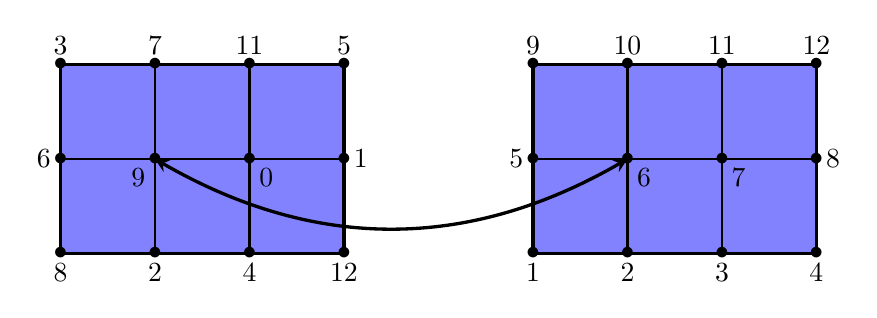
\begin{tikzpicture}[scale=1.2]

      %\draw[very thick,draw=black,fill=white!30!blue!70] (0.3,-0.15) -- (0.8,-0.15) -- (0.8,-1) -- (0.3,-1) --cycle {};
      \draw[very thick,draw=black,fill=white!30!blue!70] (0,0) -- (3,0) -- (3,2) -- (0,2) --cycle {};
      \draw[thick,draw=black] (1,0) -- (1,2);
      \draw[thick,draw=black] (2,0) -- (2,2);
      \draw[thick,draw=black] (0,1) -- (3,1);
      \draw (0,0) node {$\bullet$};
      \draw (0,0) node[below] {8};
      \draw (1,0) node {$\bullet$};
      \draw (1,0) node[below] {2};
      \draw (2,0) node {$\bullet$};
      \draw (2,0) node[below] {4};
      \draw (3,0) node {$\bullet$};
      \draw (3,0) node[below] {12};
      \draw (0,1) node {$\bullet$};
      \draw (0,1) node[left] {6};
      \draw (1,1) node {$\bullet$};
      \draw (1,1) node[below left] {9};
      \draw (2,1) node {$\bullet$};
      \draw (2,1) node[below right] {0};
      \draw (3,1) node {$\bullet$};
      \draw (3,1) node[right] {1};
      \draw (0,2) node {$\bullet$};
      \draw (0,2) node[above] {3};
      \draw (1,2) node {$\bullet$};
      \draw (1,2) node[above] {7};
      \draw (2,2) node {$\bullet$};
      \draw (2,2) node[above] {11};
      \draw (3,2) node {$\bullet$};
      \draw (3,2) node[above] {5};

    \def\shiftX{5};
      \draw[very thick,draw=black,fill=white!30!blue!70] (0+\shiftX,0) -- (3+\shiftX,0) -- (3+\shiftX,2) -- (0+\shiftX,2) --cycle {};
      \draw[thick,draw=black] (1+\shiftX,0) -- (1+\shiftX,2);
      \draw[thick,draw=black] (2+\shiftX,0) -- (2+\shiftX,2);
      \draw[thick,draw=black] (0+\shiftX,1) -- (3+\shiftX,1);
      \draw (0+\shiftX,0) node {$\bullet$};
      \draw (0+\shiftX,0) node[below] {1};
      \draw (1+\shiftX,0) node {$\bullet$};
      \draw (1+\shiftX,0) node[below] {2};
      \draw (2+\shiftX,0) node {$\bullet$};
      \draw (2+\shiftX,0) node[below] {3};
      \draw (3+\shiftX,0) node {$\bullet$};
      \draw (3+\shiftX,0) node[below] {4};
      \draw (0+\shiftX,1) node {$\bullet$};
      \draw (0+\shiftX,1) node[left] {5};
      \draw (1+\shiftX,1) node {$\bullet$};
      \draw (1+\shiftX,1) node[below right] {6};
      \draw (2+\shiftX,1) node {$\bullet$};
      \draw (2+\shiftX,1) node[below right] {7};
      \draw (3+\shiftX,1) node {$\bullet$};
      \draw (3+\shiftX,1) node[right] {8};
      \draw (0+\shiftX,2) node {$\bullet$};
      \draw (0+\shiftX,2) node[above] {9};
      \draw (1+\shiftX,2) node {$\bullet$};
      \draw (1+\shiftX,2) node[above] {10};
      \draw (2+\shiftX,2) node {$\bullet$};
      \draw (2+\shiftX,2) node[above] {11};
      \draw (3+\shiftX,2) node {$\bullet$};
      \draw (3+\shiftX,2) node[above] {12};

      \draw[<->,>=stealth,very thick] (1,1) to[bend right] (1+\shiftX,1);


    \end{tikzpicture}
  \end{figure}
\end{block}

\begin{block}{Pourquoi construire cette relation?}
  \begin{itemize}
  \item Calcul d'intégrale sur un bord ou l'ensemble du domaine
  \item Visulation de la solution différence fini
  \item projection, derivation, ... (operateurs de Feel++)
  %\item Correspondance des degrés de liberté entre E.F et D.F
  \end{itemize}
\end{block}



\end{frame}

\begin{frame}{Quelques détails d'implémentations}

\begin{block}{Discrétisation du vecteur direction}
  \begin{columns}
    \column[c]{.65\textwidth}

  \begin{itemize}
  \item Chargement d'un maillage 2d $\left[0,\pi\right] \times \left[0,2\pi\right]$  \\ ( x-coord: $\theta$, y-coord: $\phi$ )
  \item Calcul du vecteur direction à chaque noeud du maillage $\vec{v}_{ij} = F(\theta_{i},\phi_{j})$
  \end{itemize}

    \column[c]{.35\textwidth}

  \vspace*{-0.35\textwidth}
\begin{figure}[htb]
  \centering
  %,height=0.3\textheight
  \subfigure[]{
    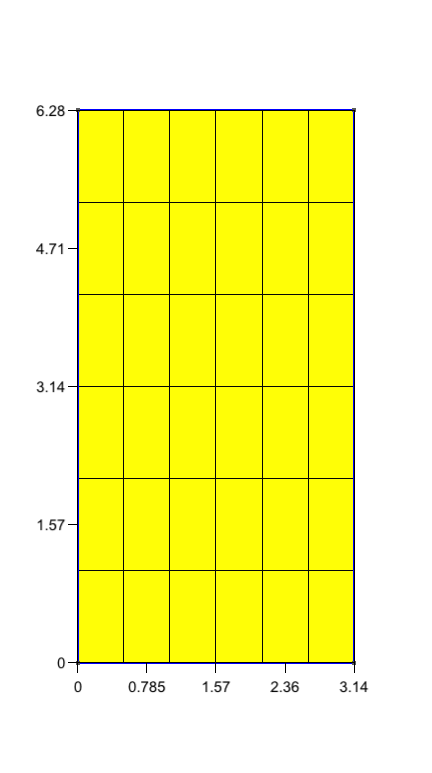
\includegraphics[width=0.4\textwidth]{Figures/acoustic-vecpropagation} 
  }
  \subfigure[]{
    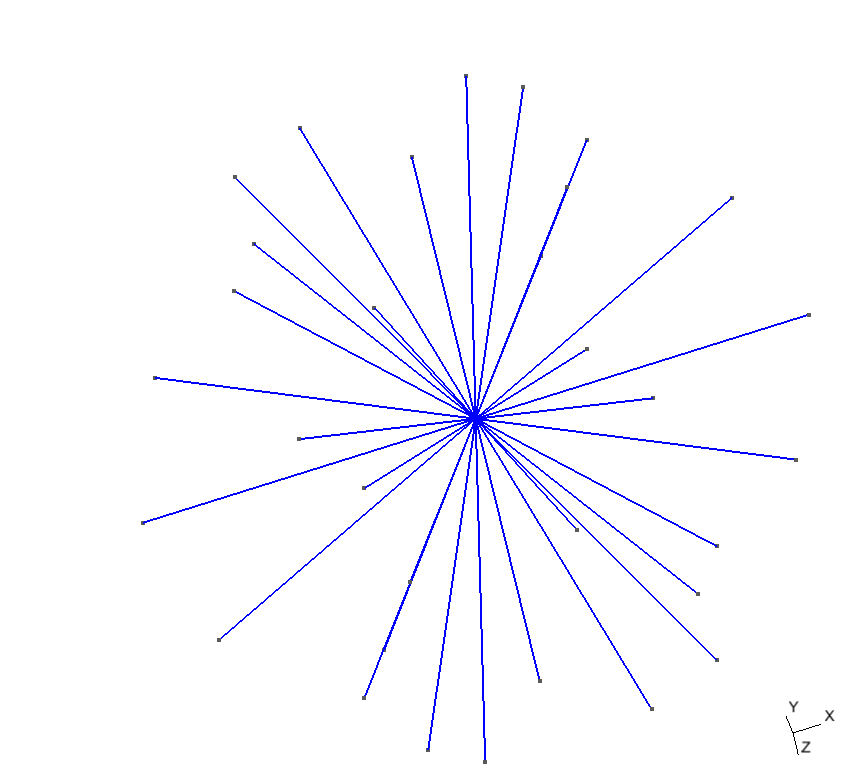
\includegraphics[width=0.4\textwidth]{Figures/allvectordirection} 
  }
\end{figure}
  \end{columns}

\end{block}

\begin{block}{Calcul de $w(\vec{r},\hat{\theta},\hat{\phi},t)$}
  \begin{itemize}
  \item Localisation du point $(\hat{\theta},\hat{\phi})=(\pi-\theta,\pi-\phi)$ dans le maillage 2d
  \item Interpolation linéaire de $w(\vec{r},\hat{\theta},\hat{\phi},t)$
  \end{itemize}
\end{block}



\end{frame}

%%%%%%%%%%%%%%%%%%%%%%%%%%%%%%%%%%%%%%%%%%%%%%%%%%%%%%%%%%%%%%%%%%%%%%%%%%%%%%


\begin{frame}{Stratégie du solveur : $Ax=F$}

\begin{itemize}
\item Méthodes de sous-espaces de Krylov :
Chercher une approximation de la solution dans un espace dont la dimension augmente à chaque étape :
%find an approximated solution in a space which the dimension increase at each step : 
\begin{equation*}
  u^{n+1} = \underbrace{u^0}_{\text{initial guess}} + \underbrace{Span\left\{ r^0,Ar^0,...,A^{n-1}r^0 \right\}}_{\text{Krylov subspace}} \quad \text{ avec } r^k=F-Ax^k
\end{equation*}
\item GMRES, CG, BICG, FGMRES, ...
\item Vitesse de convergence dépend du nombre de conditionnement de A
\item Méthodes de sous-espaces de Krylov préconditionnées :
%Transform original system into a equivalent system which have a better conditioning :
%Left preconditioning :
 $\underbrace{M_L^{-1} A}_{\tilde{A}} \ \underbrace{x}_{\tilde{x}} = \underbrace{M_L^{-1} F}_{\tilde{F}}  $
%% %\begin{itemize}
%%  Left preconditioning :
%% $\underbrace{M_L^{-1} A}_{\tilde{A}} \ \underbrace{x}_{\tilde{x}} = \underbrace{M_L^{-1} F}_{\tilde{F}}  $
%% \item Right preconditioning :
%% $ \underbrace{ A M_R^{-1}}_{\tilde{A}}  y = F $ et $x=M_R^{-1} y$

%% \item Left and right preconditioning :
%% $\underbrace{M_L^{-1} A M_R^{-1} }_{\tilde{A}}   y = \underbrace{M_L^{-1} F}_{\tilde{F}} $ et $x=M_R^{-1} y$

%% \end{itemize}

\end{itemize}

\begin{alert}{Optimisation :}
construction de la factorisation LU comme préconditionneur et réutilisation de ce préconditionneur
pour chaque direction et pour tous les pas de temps
\end{alert}



\end{frame}


%%%%%%%%%%%%%%%%%%%%%%%%%%%%%%%%%%%%%%%%%%%%%%%%%%%%%%%%%%%%%%%%%%%%%%%%%%%%%%

\begin{frame}{Applications}
\begin{itemize}
\item Equation de transport 1d, 2d et 3d : ok !
\begin{figure}[htb]
  \centering
  %,height=0.3\textheight
  \subfigure[t0]{
    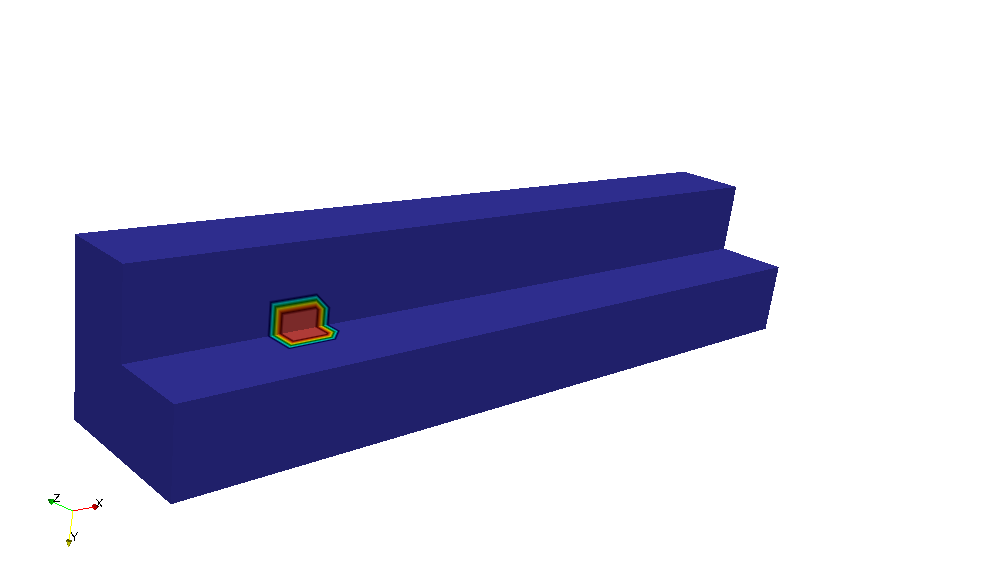
\includegraphics[width=0.25\textwidth]{Figures/simu3d_t0} 
  }
  \subfigure[t1]{
    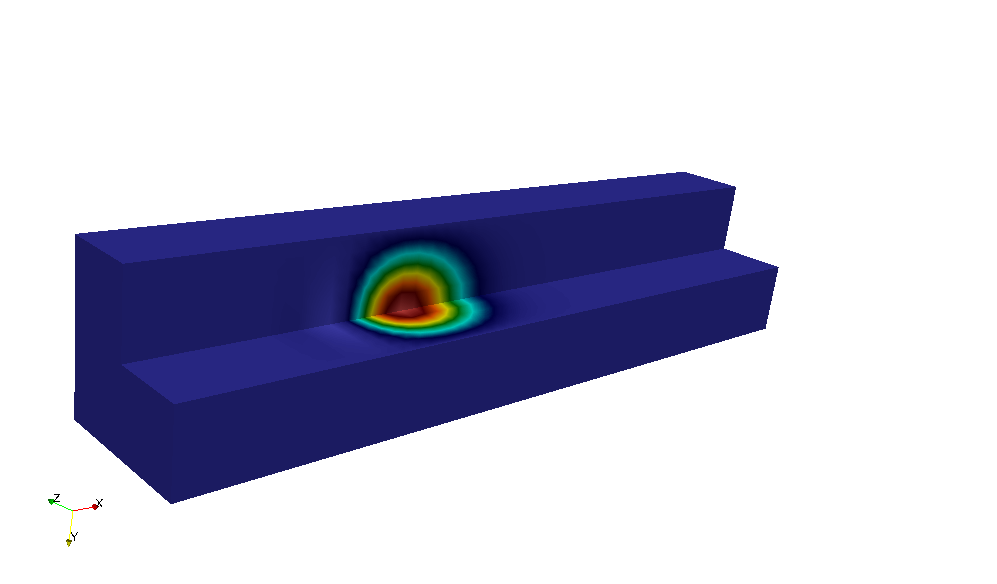
\includegraphics[width=0.25\textwidth]{Figures/simu3d_t1} 
  }
  \subfigure[t2]{
    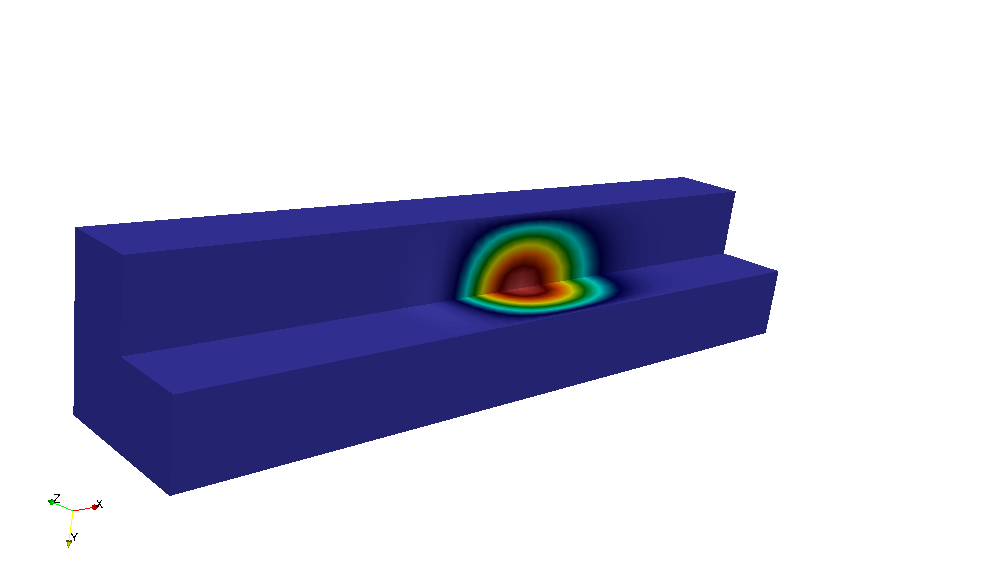
\includegraphics[width=0.25\textwidth]{Figures/simu3d_t2} 
  }
\end{figure}

\item Equation de transport 5d : %{\Huge{\danger}} bug non résolu !
\end{itemize}
\end{frame}

%%%%%%%%%%%%%%%%%%%%%%%%%%%%%%%%%%%%%%%%%%%%%%%%%%%%%%%%%%%%%%%%%%%%%%%%%%%%%%


\end{document}
